\documentclass{article}%
\usepackage{amsmath}%
\usepackage{amsfonts}%
\usepackage{amssymb}%
\usepackage{graphicx}
\usepackage[export]{adjustbox}
\usepackage{enumitem}
%-------------------------------------------
\newtheorem{theorem}{Theorem}
\newtheorem{acknowledgement}[theorem]{Acknowledgement}
\newtheorem{algorithm}[theorem]{Algorithm}
\newtheorem{axiom}[theorem]{Axiom}
\newtheorem{case}[theorem]{Case}
\newtheorem{claim}[theorem]{Claim}
\newtheorem{conclusion}[theorem]{Conclusion}
\newtheorem{condition}[theorem]{Condition}
\newtheorem{conjecture}[theorem]{Conjecture}
\newtheorem{corollary}[theorem]{Corollary}
\newtheorem{criterion}[theorem]{Criterion}
\newtheorem{definition}[theorem]{Definition}
\newtheorem{example}[theorem]{Example}
\newtheorem{exercise}[theorem]{Exercise}
\newtheorem{lemma}[theorem]{Lemma}
\newtheorem{notation}[theorem]{Notation}
\newtheorem{problem}[theorem]{Problem}
\newtheorem{proposition}[theorem]{Proposition}
\newtheorem{remark}[theorem]{Remark}
\newtheorem{solution}[theorem]{Solution}
\newtheorem{summary}[theorem]{Summary}
\newenvironment{proof}[1][Proof]{\textbf{#1.} }{\ \rule{0.5em}{0.5em}}
\setlength{\textwidth}{7.0in}
\setlength{\oddsidemargin}{-0.35in}
\setlength{\topmargin}{-0.5in}
\setlength{\textheight}{9.0in}
\setlength{\parindent}{0.3in}
\begin{document}

\begin{flushright}
\textbf{Chanjoon Park \\
Feb 10, 2024}
\end{flushright}

\begin{center}
\textbf{CS 285: Deep Reinforcement Learning, Decision Making, and Control \\
Assignment 1. Imitation Learning \\}
\end{center}

\section*{1. Analysis}

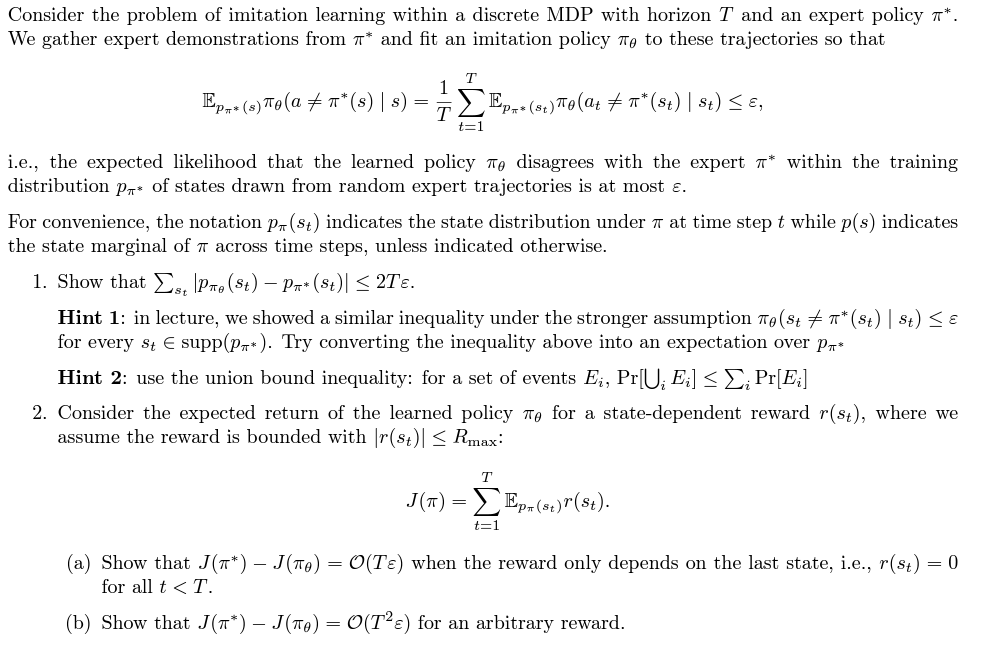
\includegraphics[width=\textwidth, center]{cs285_hw1_analysis.png}

\hrule

\section*{Solutions.}

\subsection*{1.1.}
Consider a discrete MDP, horizon $T$, an expert policy $\pi_E$, and a policy $\pi$ that is parameterized by $\theta$.

First, we have given boundaries of the expected likelihood as follows:

\begin{equation}
	\frac{1}{T}\sum_{t=1}^{T}\mathbb{E}_{p^*_\pi(s_t)}\pi_\theta(a_t \neq \pi^*(s)|s)=\frac{1}{T}\sum_{t=1}^{T}\sum_{s_t}p^*_\pi(s_t)\pi_\theta(a \neq \pi^*(s)) \leq \epsilon \\
\end{equation}

And using the union bound inequality, we can derive the following:

\begin{equation}
\sum_{s_t}p^*_\pi(s_t)\pi_\theta(a \neq \pi^*(s)) \leq \epsilon
\end{equation}

\newpage
Second, derive the probability of the policy $\pi_\theta$ like Lecture 2.

\begin{equation}
	p_{\pi_\theta}(s_t) = (1 - \epsilon)^t p_{\pi^*}(s_t) + (1 - (1 - \epsilon)^t) p_{\pi_\text{mistake}}(s_t)
\end{equation}

Finally, show that $\sum_{s_t} |p_{\pi_\theta}(s_t) - p_{\pi^*}(s_t)| \leq 2T\epsilon$.
\begin{align*}
	\sum_{s_t} |p_{\pi_\theta}(s_t) - p_{\pi^*}(s_t)| &= \sum_{s_t} |(1 - \epsilon)^t p_{\pi^*}(s_t) + (1 - (1 - \epsilon)^t) p_{\pi_\text{mistake}}(s_t) - p_{\pi^*}(s_t)| \\
	&= \sum_{s_t} |(1 - (1 - \epsilon)^t) p_{\pi_\text{mistake}}(s_t)| \\
	&\leq \sum_{s_t} (1 - (1-\epsilon t)) |p_{\pi_\text{mistake}}(s_t) - p_{\pi^*}(s_t)| \quad (\because (1-\epsilon)^t \geq 1-\epsilon t\ \text{for}\ \epsilon \in [0, 1])\\
	&\leq \sum_{s_t} 2(1 - (1-\epsilon t)) = \sum_{s_t} 2\epsilon t = 2T\epsilon \quad (\because \sum_{s_t}t = T)
\end{align*}

\textbf{Note}: I assumed that sum of $t$ over $s_t$ is same as $T$.

\subsection*{1.2.}

\begin{enumerate}[label=(\alph*)]
	\item Show that $J(\pi^*) - J(\pi_\theta)=O(T\epsilon)$ when $r(s_t) = 0 \text{ for all } t < T$
	
	\begin{align*}
		J(\pi^*) - J(\pi_\theta) &= \sum_{t=1}^{T} \mathbb{E}_{p^*_\pi}(s_t)r(s_t) - \sum_{t=1}^{T} \mathbb{E}_{p_{\pi_\theta}}(s_t)r(s_t) \\
		&= \sum_{t=1}^{T} \Big(\sum_{s_t}(p_{\pi^*}(s_t) - p_{\pi_\theta}(s_t))r(s_t)\Big) \\
		&=(p_{\pi^*}(s_T) - p_{\pi_\theta}(s_T))r(s_T) \leq 2T\epsilon R_{\max} 
	\end{align*}
	
	Thus, $J(\pi^*) - J(\pi_\theta)=O(T\epsilon)$
	
	\item Show that $J(\pi^*) - J(\pi_\theta)=O(T^2 \epsilon)$ for an arbitrary reward.
	
	\begin{align*}
		J(\pi^*) - J(\pi_\theta) &= \sum_{t=1}^{T} \mathbb{E}_{p^*_\pi}(s_t)r(s_t) - \sum_{t=1}^{T} \mathbb{E}_{p_{\pi_\theta}}(s_t)r(s_t) \\
		&= \sum_{t=1}^{T} \Big(\sum_{s_t}(p_{\pi^*}(s_t) - p_{\pi_\theta}(s_t))r(s_t)\Big) \\
		& \leq \sum_{t=1}^{T} \Big(\sum_{s_t} | p_{\pi^*}(s_t) - p_{\pi_\theta}(s_t) | \cdot R_{max} \Big) \\
		& \leq \sum_{t=1}^{T} 2T\epsilon R_{max} = 2T^2 \epsilon R_{max}
	\end{align*}

	Thus, $J(\pi^*) - J(\pi_\theta)=O(T^2 \epsilon)$
\end{enumerate}

\end{document}
% https://www.overleaf.com/latex/templates/computer-science-homework-template/cktrjmbzsqpt